
\section{Certificaciones de SCRUM MASTER}
\begin{frame}[allowframebreaks]{Certificaciones de SCRUM MASTER}
	
	Scrum y Scrum Master
	
	\begin{itemize}
		\item \textbf{Scrum} es un marco de trabajo ágil para desarrollar y mantener productos complejos.
		\item \textbf{Scrum Master} es la persona conocedora del proceso SCRUM.
	\end{itemize}


	Las dos principales \textbf{organizaciones certificadoras} son:
	\begin{itemize}
		\item Scrum Alliance (Certificación CSM)
		\item Scrum.org (Certificación PSM)
	\end{itemize}

\end{frame}

\subsection{Certificación CSM}

\begin{frame}{Certificación CSM}
	Certificación \textbf{CSM} \foreign{Certified Scrum Master}
	\begin{itemize}
		\item \textbf{Curso obligatorio} de 16 horas.
		\item \textbf{Examen on-line} obligatorio de 35 preguntas verdadero/falso y de múltiple opción.
		\item \textbf{Renovaciones obligatorias} cada dos años.
	\end{itemize}

	\begin{center}
		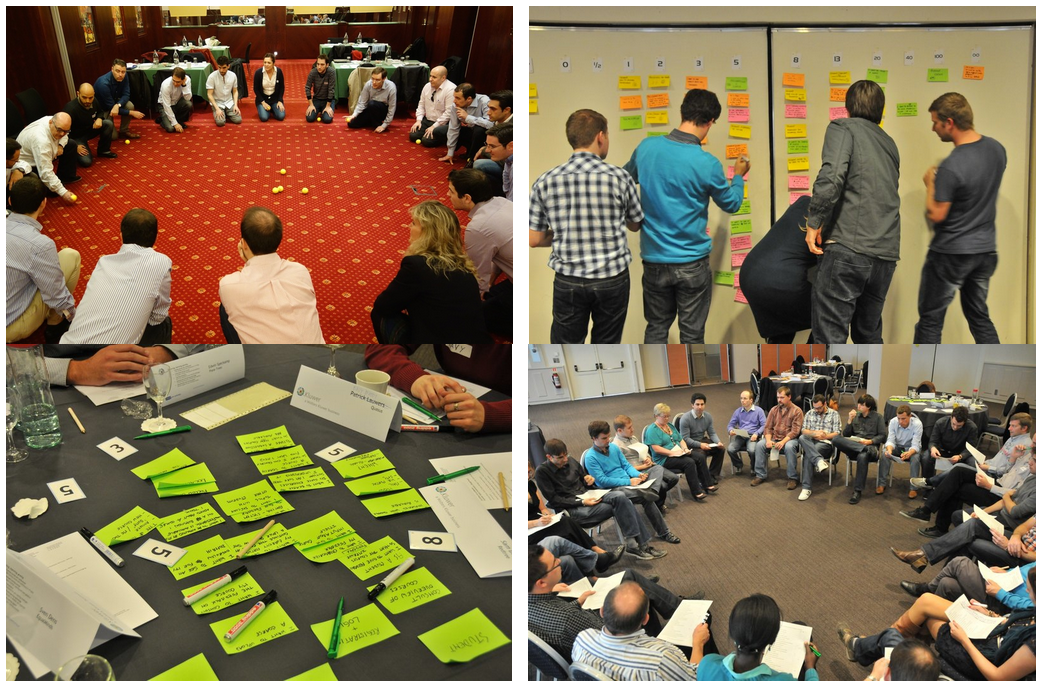
\includegraphics[height=3.5cm]{figuras/curso_scrum.png}
	\end{center}

\end{frame}

\subsection{Certificación PSM}

\begin{frame}[allowframebreaks]{Certificación PSM}
	Certificación \textbf{PSM} \foreign{Proffesional Scrum Master}

	\begin{itemize}
		\item Consta de tres niveles de certificación PSM I, PSM II y PSM III
		\item No requiere la realización de ningún curso.
		\item \textbf{No requiere de renovaciones}.
	\end{itemize}

	\framebreak

	Certificación PSM I
	\begin{itemize}
		\item Conocimiento \textbf{básico} sobre las funciones del Scrum Master.
		\item Evaluación basada en \textbf{The Scrum Guide}
		\item Examen de una hora con 80 preguntas de múltiple elección y
		      verdadero/falso.
		\item La evaluación cuesta \$150
	\end{itemize}

	\framebreak

	Certificación PSM II
	\begin{itemize}
		\item Conocimiento \textbf{avanzado} sobre las funciones de un Scrum Master
		\item Examen de 90 minutos 30 preguntas de múltiple elección,
		      múltiple respuesta o  verdadero/falso
		\item La evaluación cuesta \$250
	\end{itemize}

	\framebreak

	Certificación PSM III
	\begin{itemize}
		\item Conocimiento \textbf{distinguido} sobre las tareas 
		      del Scrum Master.
		\item Examen de 2 horas Preguntas de múltiple elección y 
		      \textbf{casos prácticos}.
		\item Requiere haber superado las certificaciones PSM I y PSM II
		\item La evaluación cuesta \$500
	\end{itemize}


\end{frame}


\section{La guía del PMBOK: Introducción.}

\subsection{Propósito}
\begin{frame}{Propósito}
	
	\begin{itemize}
		\item{Identifica un conjunto de \textbf{buenas prácticas} para la dirección de proyectos}
		\item{Proporciona un vocabulario común para los conceptos de la dirección de proyectos}
		\item{\textbf{Es una guía, no una metodología}}
	\end{itemize}
\end{frame}

%%
% ahora explicas que los dos primeros capítulos de la guía PMBOK
% son una introducción a una serie de conceptos importantes en el 
% ámbito de la dirección de proyectos, y que hablaremos de algunos
% que hemos considerado más interesantes.
%%
\subsection{Portafolios, Programas y Proyectos}
\begin{frame}[allowframebreaks]{Portafolios, Programas y Proyectos}
	
	\begin{block}{Definición de Portafolios}
		Un portafolio es un grupo de proyectos, programas, subgrupos de  portafolios y operaciones, que son gestionadas como un conjunto, con el fin de alcanzar los objetivos estratégicos de la empresa.
	\end{block}

	% ejemplos de estrategias de empresa pueden ser por ejemplo 
	% "maximizar el rendimiento de las inversiones"

	\framebreak

	\begin{block}{Definición de Programa}
		Un programa es un grupo de proyectos relacionados, subprogramas y actividades de programas, cuya gestión se realiza de forma coordinada para obtener beneficios que no se obtendrían si se gestionaran de forma individual.
	\end{block}

	% todo : buscar ejemplos de programa para explicarlo

	\framebreak
	\begin{center}
		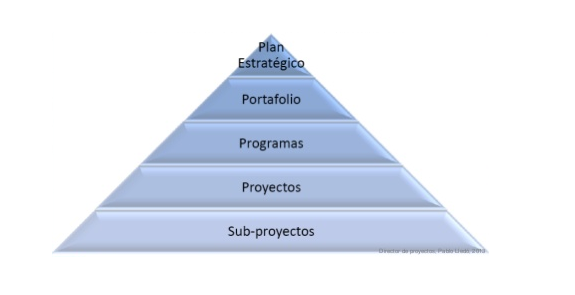
\includegraphics[height=5cm]{figuras/proy_prog_port_00.png}

		Contexto de la dirección de proyectos
	\end{center}

\end{frame}


\subsection{El ciclo de vida del proyecto}
\begin{frame}{El ciclo de vida del proyecto}
	
	El ciclo de vida es la serie de fases por las que pasa un proyecto desde su inicio hasta su cierre, proporcionando un marco de referencia básico para dirigir el proyecto.

	\begin{center}
		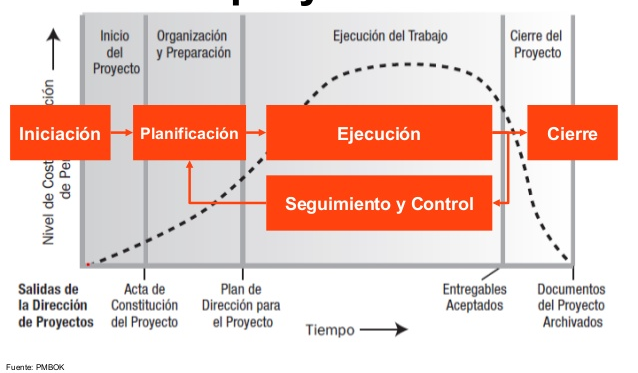
\includegraphics[height=4.5cm]{figuras/ciclo_vida_00.png}

		Estructura genérica de ciclo de vida.
	\end{center}


	

\end{frame}

